\documentclass[11pt,a4paper]{article}
\usepackage[T1]{fontenc}
\usepackage[utf8]{inputenc}
\usepackage{lmodern}
\usepackage{textcomp}
\usepackage[left=1.8cm,right=1.8cm,top=2.3cm,bottom=2.2cm,headheight=14pt,headsep=8pt]{geometry}
\usepackage{multicol}
\usepackage{xcolor}
\usepackage{fancyhdr}
\usepackage{graphicx}
\usepackage{array}
\usepackage{amsmath,amssymb}
\usepackage{setspace}
\usepackage{longtable}
\graphicspath{{../}}
\definecolor{ygreen}{RGB}{46,139,87}
\renewcommand{\normalsize}{\fontsize{10.9}{13.4}\selectfont}
\renewcommand{\familydefault}{\rmdefault}
\setlength{\parindent}{0pt}
\setlength{\columnsep}{0.8cm}
\setlength{\columnseprule}{0.4pt}
\setlength{\multicolsep}{3pt plus 1pt minus 1pt}
\renewcommand{\textsubscript}[1]{\ensuremath{_{\text{\fontsize{8}{8}\selectfont #1}}}}
\renewcommand{\textsuperscript}[1]{\ensuremath{^{\text{\fontsize{8}{8}\selectfont #1}}}}
\newcommand{\qn}[1]{\textbf{\fontsize{11.5}{13}\selectfont #1}}
\newcommand{\qsep}{\par\vspace{1pt}\noindent\rule{0pt}{0.4pt}\par\vspace{5pt}}
\newcommand{\fwrule}{\par\vspace{5pt}\noindent\rule{\linewidth}{1.4pt}\par\vspace{7pt}}
\newsavebox{\fitb}
\newcommand{\fitbox}[1]{\sbox{\fitb}{#1}\ifdim\wd\fitb>\linewidth\resizebox{\linewidth}{!}{\usebox{\fitb}}\else\usebox{\fitb}\fi}
\newcommand{\diqqat}[1]{\par\smallskip\noindent\textbf{Diqqat!} #1\par\medskip}
\newcommand{\javob}{\par\smallskip\noindent\textbf{Javob:} \rule[-2pt]{7.5cm}{0.4pt}\par\smallskip\noindent\textbf{Diqqat!} Javobingizni javoblar varaqasiga ko`chirib yozing.\par\medskip}
\pagestyle{fancy}
\fancyhf{}
\renewcommand{\headrulewidth}{0.4pt}
\fancyhead[L]{\textit{Milliy sertifikat 2026. Kimyo}}
\fancyhead[R]{19-variant}
\fancyfoot[L]{\fontsize{8}{9}\selectfont \textcopyright{} Colba maktabi, 2026}
\fancyfoot[C]{\thepage}
\fancypagestyle{first}{\fancyhf{}\renewcommand{\headrulewidth}{0pt}\fancyfoot[L]{\fontsize{8}{9}\selectfont \textcopyright{} Colba maktabi, 2026}\fancyfoot[C]{\thepage}}
\begin{document}
\normalsize
\thispagestyle{first}
\noindent\fcolorbox{ygreen}{white}{\parbox{\dimexpr\linewidth-2\fboxsep-2\fboxrule\relax}{%
\textbf{\fontsize{13}{15}\selectfont Nazorat testi}\ \textit{\fontsize{10}{12}\selectfont $\cdot$ Aralash test $\cdot$ 19-variant}\hfill
\begin{tabular}[t]{@{}r@{}}\textit{Milliy sertifikat 2026. Kimyo}\\ \textbf{\textit{\fontsize{8}{9}\selectfont Vaqt:}} \textit{\fontsize{10}{12}\selectfont 180 daqiqa}\end{tabular}}}
\par\medskip
\noindent\textit{Davriy jadvaldan foydalanish mumkin.}
\par\medskip
\begin{multicols}{2}
\noindent\qn{1.} AgNO\textsubscript{3} eritmasi inert elektrodlar yordamida 4 A tok kuchi bilan 965 s elektroliz qilindi. Anodda ajralgan O\textsubscript{2} hajmi (l, n.sh.) \textbf{ni toping.}

\noindent A)~\textsl{0,448} \hfill B)~\textsl{0,112} \hfill C)~\textsl{0,009} \hfill D)~\textsl{0,224}\par
\qsep
\noindent\qn{2.} Xrom atomida d-pog`onachadagi elektronlar \textbf{sonini aniqlang} (\textit{Z} = 24).

\noindent A)~\textsl{5} \hfill B)~\textsl{6} \hfill C)~\textsl{4} \hfill D)~\textsl{7}\par
\qsep
\noindent\qn{3.} Mishyak (\textit{Z} = 33) atomining tashqi energetik pog`onasidagi elektronlar \textbf{sonini aniqlang.}

\noindent A)~\textsl{5} \hfill B)~\textsl{6} \hfill C)~\textsl{4} \hfill D)~\textsl{7}\par
\qsep
\noindent\qn{4.} Quyidagi tuzlarning qaysilari suvli eritmasi ishqoriy muhitga ega? 1) CH\textsubscript{3}COONa; 2) FeCl\textsubscript{3}; 3) K\textsubscript{2}S; 4) NH\textsubscript{4}Cl

\noindent A)~\textsl{2, 3, 4} \hfill B)~\textsl{1, 3} \hfill C)~\textsl{2, 3} \hfill D)~\textsl{3}\par
\qsep
\noindent\qn{5.} 2 mol Ba(OH)\textsubscript{2} va 2 mol NaCl suvda eritilib, eritma hajmi 4 l ga yetkazildi. Eritmadagi barcha ionlarning umumiy molyar \textbf{konsentratsiyasini (mol/l) aniqlang} (kuchli elektrolitlar to`liq dissotsilanadi).

\noindent A)~\textsl{1} \hfill B)~\textsl{5} \hfill C)~\textsl{2,5} \hfill D)~\textsl{1,25}\par
\qsep
\noindent\qn{6.} Kislotada Mg bo`lagi eritilganda ajralgan vodorod hajmining vaqtga bog`liqligi grafikda berilgan.
\begin{center}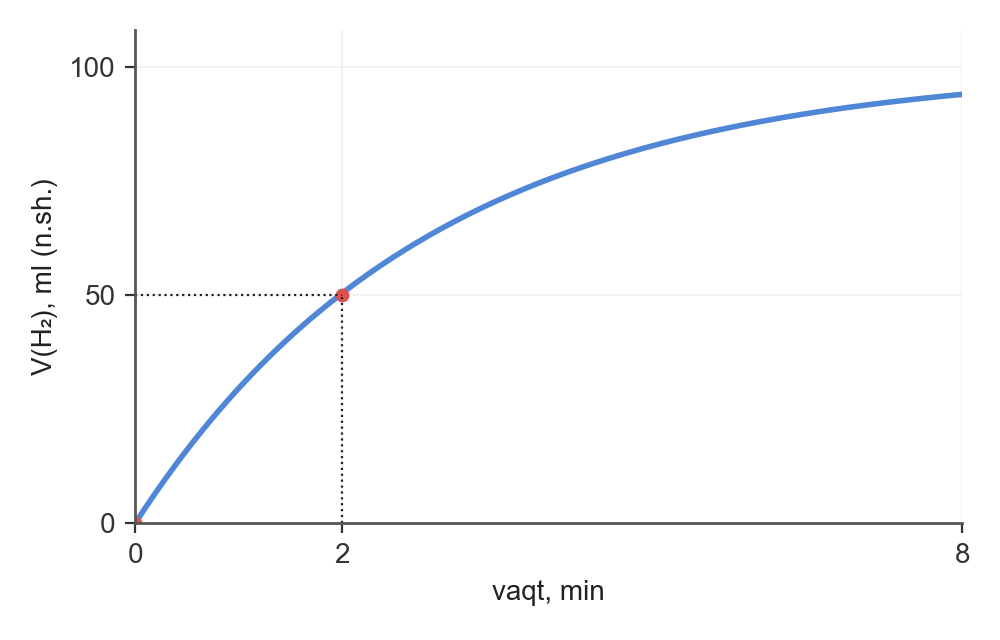
\includegraphics[width=0.86\linewidth]{rasmlar/gen/gv_v19_0.png}\end{center}
2-minutda ajralgan vodorodning \textbf{miqdorini (mmol) toping} (1 mmol gaz = 22,4 ml).

\noindent A)~\textsl{2,23} \hfill B)~\textsl{4,46} \hfill C)~\textsl{1,12} \hfill D)~\textsl{50}\par
\qsep
\noindent\qn{7.} Laboratoriyada CuSO\textsubscript{4} eritmalari quyidagicha tayyorlangan:
\begin{center}
\renewcommand{\arraystretch}{1.15}
\fitbox{\begin{tabular}{|c|c|c|}\hline
\textbf{Idish} & \textbf{Eritma massasi, g} & \textbf{$\omega$(CuSO\textsubscript{4}), \%} \\ \hline
A & 200 & 5 \\ \hline
B & 150 & 40 \\ \hline
\end{tabular}}
\end{center}
Bu ikki eritma bir idishga quyilib, yangi eritmadagi CuSO\textsubscript{4} ning massa ulushi (\%) qancha bo`ladi?

\noindent A)~\textsl{22,5} \hfill B)~\textsl{45} \hfill C)~\textsl{20} \hfill D)~\textsl{25}\par
\qsep
\noindent\qn{8.} Jadvalda bog`lar hosil qiluvchi atomlarning elektrmanfiyliklari berilgan:
\begin{center}
\renewcommand{\arraystretch}{1.15}
\fitbox{\begin{tabular}{|c|c|c|}\hline
\textbf{Bog`} & \textbf{EM (1-atom)} & \textbf{EM (2-atom)} \\ \hline
H--N & 2,1 & 3 \\ \hline
Mg--O & 1,2 & 3,5 \\ \hline
C--H & 2,5 & 2,1 \\ \hline
Si--O & 1,8 & 3,5 \\ \hline
\end{tabular}}
\end{center}
Qaysi bog` eng qutbli (eng ko`p ionli xarakterga ega)?

\noindent A)~\textsl{H--N} \hfill B)~\textsl{C--H} \hfill C)~\textsl{Si--O} \hfill D)~\textsl{Mg--O}\par
\qsep
\noindent\qn{9.} 8 g NaOH va 5,48 g HCl aralashtirilib, reaksiya o`tkazildi (NaOH + HCl $\to$ NaCl + H\textsubscript{2}O). Hosil bo`lgan NaCl \textbf{massasini (g) aniqlang.}

\noindent A)~\textsl{11,7} \hfill B)~\textsl{17,55} \hfill C)~\textsl{4,39} \hfill D)~\textsl{8,78}\par
\qsep
\noindent\qn{10.} 131,2 l N\textsubscript{2} 127 \textdegree{}C va 0,5 atm bosimda necha gramm keladi? (R = 0,082 l$\cdot$atm/(mol$\cdot$K))

\noindent A)~\textsl{112} \hfill B)~\textsl{56} \hfill C)~\textsl{28} \hfill D)~\textsl{164}\par
\qsep
\noindent\qn{11.} HC$\equiv$C--CH=CH\textsubscript{2} molekulasidagi $\sigma$ va $\pi$ bog`lar \textbf{sonini aniqlang.}

\noindent A)~\textsl{6 va 3} \hfill B)~\textsl{7 va 4} \hfill C)~\textsl{8 va 3} \hfill D)~\textsl{7 va 3}\par
\qsep
\noindent\qn{12.} K\textsubscript{2}Cr\textsubscript{2}O\textsubscript{7} tarkibida Cr ning oksidlanish \textbf{darajasini aniqlang.}

\noindent A)~\textsl{$-$1} \hfill B)~\textsl{+1} \hfill C)~\textsl{+6} \hfill D)~\textsl{$-$3}\par
\qsep
\noindent\qn{13.} Faqat qaytaruvchi bo`la oladigan \textbf{ionlarni aniqlang}: 1) Al\textsuperscript{3+}; 2) S\textsuperscript{2$-$}; 3) Na\textsuperscript{+}; 4) Fe\textsuperscript{3+}

\noindent A)~\textsl{1, 4} \hfill B)~\textsl{1, 3} \hfill C)~\textsl{3, 4} \hfill D)~\textsl{2}\par
\qsep
\noindent\qn{14.} Reaksiya tenglamasi: SiO\textsubscript{2} + 2NaOH $\to$ Na\textsubscript{2}SiO\textsubscript{3} + H\textsubscript{2}O. Reaksiyaga tarkibida 20\% aralashma bo`lgan 20 g namuna (asosiy modda NaOH) kirishdi. Na\textsubscript{2}SiO\textsubscript{3} \textbf{massasini (g) hisoblang.}

\noindent A)~\textsl{97,6} \hfill B)~\textsl{48,8} \hfill C)~\textsl{24,4} \hfill D)~\textsl{12,2}\par
\qsep
\noindent\qn{15.} 2NaBr + Cl\textsubscript{2} $\to$ 2NaCl + Br\textsubscript{2} reaksiyasida 71 g Cl\textsubscript{2} ishtirok etdi. Br\textsubscript{2} \textbf{miqdorini (mol) toping.}

\noindent A)~\textsl{1} \hfill B)~\textsl{2} \hfill C)~\textsl{0,5} \hfill D)~\textsl{1,5}\par
\qsep
\noindent\qn{16.} Ishqoriy metallar haqida qaysi fikrlar to`g`ri? 1) KOH -- kuchli ishqor; 2) Natriy atomining tashqi qavatida 2 ta elektron bor; 3) Natriy kerosin ostida saqlanadi; 4) Natriy suv bilan reaksiyada H\textsubscript{2} va NaOH hosil qiladi

\noindent A)~\textsl{1, 2, 3} \hfill B)~\textsl{1, 3, 4} \hfill C)~\textsl{2, 3} \hfill D)~\textsl{1, 2, 4}\par
\qsep
\noindent\qn{17.} Mg\textsubscript{3}N\textsubscript{2} + 6H\textsubscript{2}O $\to$ 3Mg(OH)\textsubscript{2} + 2NH\textsubscript{3} jarayoni uchun 50 g Mg\textsubscript{3}N\textsubscript{2} olingan (unum 90\%). NH\textsubscript{3} \textbf{hajmini (l, n.sh.) aniqlang.}

\noindent A)~\textsl{5,6} \hfill B)~\textsl{40,32} \hfill C)~\textsl{20,16} \hfill D)~\textsl{10,08}\par
\qsep
\noindent\qn{18.} 4,5 g Fe(OH)\textsubscript{2} havoda to`liq oksidlanib, Fe(OH)\textsubscript{3} ga aylandi. Hosil bo`lgan Fe(OH)\textsubscript{3} \textbf{massasini (g) aniqlang.}

\noindent A)~\textsl{4,5} \hfill B)~\textsl{5,35} \hfill C)~\textsl{8,03} \hfill D)~\textsl{4,95}\par
\qsep
\noindent\qn{19.} Ca(HCO\textsubscript{3})\textsubscript{2} + Ca(OH)\textsubscript{2} $\to$ 2CaCO\textsubscript{3} + 2H\textsubscript{2}O reaksiyasida 40,5 g Ca(HCO\textsubscript{3})\textsubscript{2} ishtirok etdi (unum 50\%). CaCO\textsubscript{3} \textbf{massasini (g) toping.}

\noindent A)~\textsl{12,5} \hfill B)~\textsl{50} \hfill C)~\textsl{25} \hfill D)~\textsl{37,5}\par
\qsep
\noindent\qn{20.} C\textsubscript{4}H\textsubscript{6} alkinlarning izomerlari soni nechta?

\noindent A)~\textsl{3} \hfill B)~\textsl{1} \hfill C)~\textsl{4} \hfill D)~\textsl{2}\par
\qsep
\noindent\qn{21.} CH\textsubscript{2}=CH--CH=CH\textsubscript{2} birikmaning sistematik nomi qaysi qatorda to`g`ri keltirilgan?

\noindent\begin{tabular}{@{}p{0.47\linewidth}@{}p{0.47\linewidth}@{}}
A)~\textsl{butadiyen-1,3} & B)~\textsl{butadiyen-1,2} \\
C)~\textsl{buten-1} & D)~\textsl{butin-1} \\
\end{tabular}\par
\qsep
\noindent\qn{22.} C\textsubscript{6}H\textsubscript{6} + HNO\textsubscript{3} $\to$ C\textsubscript{6}H\textsubscript{5}NO\textsubscript{2} + H\textsubscript{2}O reaksiyasida 156 g C\textsubscript{6}H\textsubscript{6} ishtirok etdi. HNO\textsubscript{3} \textbf{massasini (g) toping.}

\noindent A)~\textsl{252} \hfill B)~\textsl{63} \hfill C)~\textsl{126} \hfill D)~\textsl{189}\par
\qsep
\noindent\qn{23.} Spirt va fenollar haqida qaysi fikrlar to`g`ri? 1) Etilenglikol zaharsiz; 2) Etanol natriy bilan reaksiyaga kirishadi; 3) Glitserin Cu(OH)\textsubscript{2} bilan ko`k kompleks hosil qiladi; 4) Fenol Cu(OH)\textsubscript{2} ni eritib ko`k kompleks hosil qiladi

\noindent A)~\textsl{2, 3} \hfill B)~\textsl{4} \hfill C)~\textsl{3, 4} \hfill D)~\textsl{2, 4}\par
\qsep
\noindent\qn{24.} Aldegid va ketonlar haqida qaysi fikrlar to`g`ri? 1) Formalin --- formaldegidning 40\% li eritmasi; 2) Ketonlar kuchsiz oksidlovchilar bilan oksidlanmaydi; 3) Aldegidlar qaytarilganda ikkilamchi spirt hosil bo`ladi; 4) Aldegidlar "kumush ko`zgu" reaksiyasini beradi

\noindent A)~\textsl{2, 3} \hfill B)~\textsl{1, 3} \hfill C)~\textsl{1, 3, 4} \hfill D)~\textsl{1, 2, 4}\par
\qsep
\noindent\qn{25.} C\textsubscript{4}H\textsubscript{8} alkenlarning izomerlari soni (sis-trans izomerlar bilan, siklik bo`lmagan) nechta?

\noindent A)~\textsl{5} \hfill B)~\textsl{3} \hfill C)~\textsl{6} \hfill D)~\textsl{4}\par
\qsep
\noindent\qn{26.} CH\textsubscript{3}COOH + C\textsubscript{2}H\textsubscript{5}OH $\to$ CH\textsubscript{3}COOC\textsubscript{2}H\textsubscript{5} + H\textsubscript{2}O reaksiyasida 120 g CH\textsubscript{3}COOH ishtirok etdi. CH\textsubscript{3}COOC\textsubscript{2}H\textsubscript{5} \textbf{massasini (g) toping.}

\noindent A)~\textsl{176} \hfill B)~\textsl{352} \hfill C)~\textsl{88} \hfill D)~\textsl{264}\par
\qsep
\noindent\qn{27.} Uglevodlar haqida qaysi fikrlar to`g`ri? 1) Kraxmal va selluloza bir xil M ga ega; 2) Kraxmal yod bilan ko`k rang beradi; 3) Saxaroza Feling suyuqligini qaytaradi; 4) Fruktoza ketospirt

\noindent A)~\textsl{2, 4} \hfill B)~\textsl{2} \hfill C)~\textsl{1, 2} \hfill D)~\textsl{1, 3, 4}\par
\qsep
\noindent\qn{28.} Rasmda benzol hosilasining tuzilish formulasi berilgan.
\begin{center}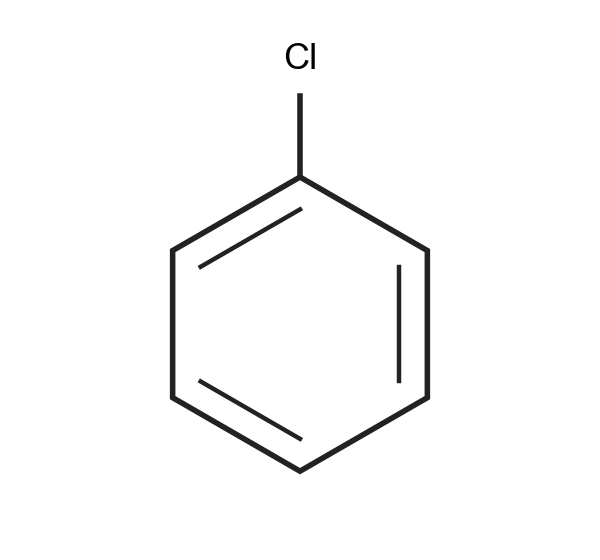
\includegraphics[width=0.86\linewidth]{rasmlar/gen/bs_14476.png}\end{center}
Birikmaning molekulyar \textbf{formulasini aniqlang.}

\noindent A)~\textsl{C\textsubscript{7}H\textsubscript{6}O\textsubscript{2}} \hfill B)~\textsl{C\textsubscript{6}H\textsubscript{5}NO\textsubscript{2}} \hfill C)~\textsl{C\textsubscript{6}H\textsubscript{5}Cl} \hfill D)~\textsl{C\textsubscript{6}H\textsubscript{6}O}\par
\qsep
\noindent\qn{29.} Reaksiya tenglamasi: C\textsubscript{2}H\textsubscript{2} + HCl $\to$ C\textsubscript{2}H\textsubscript{3}Cl. Reaksiyaga 5,2 g C\textsubscript{2}H\textsubscript{2} kirishdi. C\textsubscript{2}H\textsubscript{3}Cl \textbf{miqdorini (mol) hisoblang.}

\noindent A)~\textsl{0,4} \hfill B)~\textsl{0,2} \hfill C)~\textsl{0,1} \hfill D)~\textsl{0,3}\par
\qsep
\noindent\qn{30.} Eritmaga NaOH qo`shilganda havorang cho`kma (Cu(OH)\textsubscript{2}) kuzatildi. Eritmada qaysi ion bor?

\noindent A)~\textsl{PO\textsubscript{4}\textsuperscript{3$-$}} \hfill B)~\textsl{Cu\textsuperscript{2+}} \hfill C)~\textsl{Cl\textsuperscript{$-$}} \hfill D)~\textsl{Fe\textsuperscript{3+}}\par
\qsep
\noindent\qn{31.} Lakmus indikatori neytral muhitda qanday rang beradi?
\noindent A)~\textsl{ko`k}\par
\noindent B)~\textsl{binafsha}\par
\noindent C)~\textsl{malina rangga kiradi (pushti)}\par
\noindent D)~\textsl{qizil}\par
\qsep
\noindent\qn{32.} Rasmdagi asbobda 23 g etanol konsentrlangan H\textsubscript{2}SO\textsubscript{4} bilan 170 \textdegree{}C da qizdirilib, 90\% unum bilan etilen olindi. Hosil bo`lgan etilen \textbf{hajmini (l, n.sh.) aniqlang.}
\begin{center}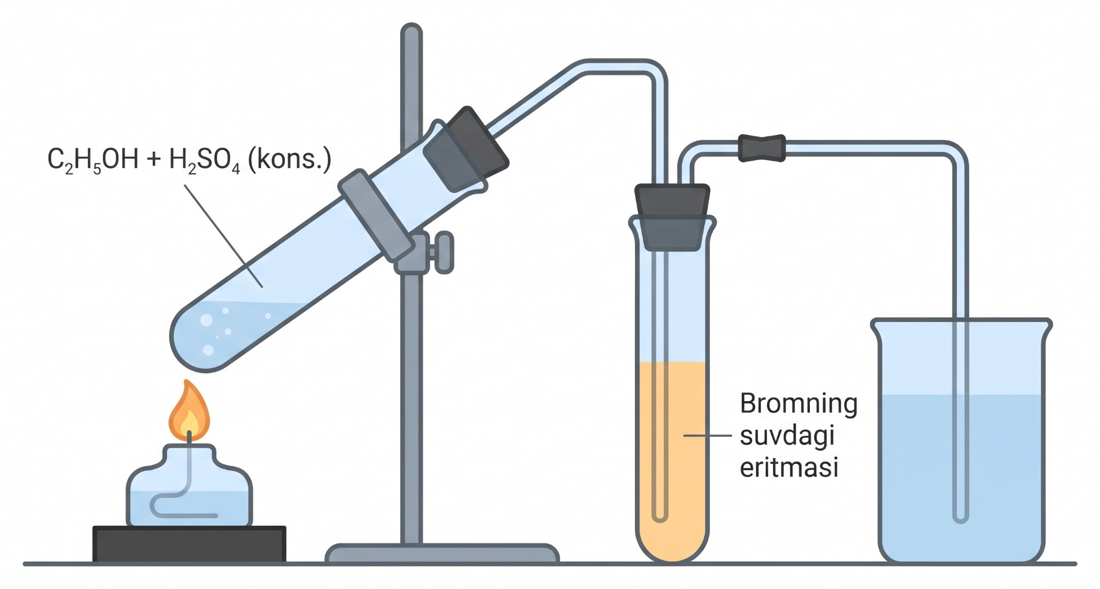
\includegraphics[width=0.86\linewidth]{rasmlar/darslik/d_etilen.png}\end{center}

\noindent\begin{tabular}{@{}p{0.47\linewidth}@{}p{0.47\linewidth}@{}}
A)~\textsl{11,2} & B)~\textsl{10,08} \\
C)~\textsl{20,16} & D)~\textsl{5,04   ---} \\
\end{tabular}\par
\qsep
\end{multicols}
\medskip
\noindent\setlength{\fboxsep}{0pt}\fbox{\begin{tabular}{p{0.74\linewidth}|p{0.2\linewidth}}
\parbox[t]{0.72\linewidth}{\vspace{3pt}\textbf{Topshiriqlar (33--35) va javob variant (A--F)larini o`zaro to`g`ri moslashtiring.} Rux va temir (Zn va Fe) dan iborat 20,05 g qotishma mo`l HCl eritmasida eritilganda 7,84 l (n.sh.) gaz ajraldi.
\vspace{3pt}} & \parbox[t]{0.19\linewidth}{\vspace{3pt}A~\textsl{67,35}\\[3pt]
B~\textsl{35,92}\\[3pt]
C~\textsl{24,31}\\[3pt]
D~\textsl{127,75}\\[3pt]
E~\textsl{44,9}\\[3pt]
F~\textsl{16,21}}\\ \hline
\parbox[t]{0.72\linewidth}{\vspace{2pt}\textbf{33. Qotishmadagi Zn massa ulushini (\%) aniqlang.}\vspace{2pt}} & \\ \hline
\parbox[t]{0.72\linewidth}{\vspace{2pt}\textbf{34. Reaksiya uchun sarflangan 20\% li HCl massasini (g) aniqlang.}\vspace{2pt}} & \\ \hline
\parbox[t]{0.72\linewidth}{\vspace{2pt}\textbf{35. Eritmadagi tuzlarning umumiy massasini (g) aniqlang.}\vspace{2pt}} & 
\end{tabular}}
\par\bigskip
\noindent\qn{36.} H\textsubscript{2}S + HNO\textsubscript{3} $\to$ H\textsubscript{2}SO\textsubscript{4} + NO\textsubscript{2} + H\textsubscript{2}O reaksiya tenglamasini elektron balans usulida tenglang va barcha koeffitsiyentlar \textbf{yig`indisini aniqlang.}
\javob\qsep
\noindent\qn{37.} CH\textsubscript{4} va H\textsubscript{2} dan iborat 60 ml aralashma mo`l kisloroda yondirildi (suv suyuq holatda; hajmlar bir xil sharoitda o`lchandi). Reaksiyadan so`ng gazlar hajmi 105 ml ga kamaydi. Aralashmadagi CH\textsubscript{4} \textbf{hajmini (ml) toping.}
\javob\qsep
\noindent\qn{38.} Al, Fe va Cu dan iborat aralashma mo`l NaOH eritmasi bilan ta'sirlashganda 6,72 l (n.sh.) vodorod ajraldi; xuddi shunday massadagi aralashma mo`l HCl bilan ta'sirlashganda 11,2 l (n.sh.) vodorod ajraldi, erimay qolgan qoldiq (mis) massasi 6,4 g. Aralashmaning dastlabki \textbf{massasini (g) toping.}
\javob\qsep
\noindent\qn{39.} 23 g etanol avval sirka aldegidgacha (unum 90\%), so`ng sirka kislotagacha (unum 80\%) oksidlandi; hosil bo`lgan kislota mo`l etanol bilan efirlandi (unum 100\%). Etilatsetat \textbf{massasini (g) toping.}
\javob\qsep
\noindent\qn{40.} 18 g sirka kislota va 9,2 g etanol dan 80\% unum bilan murakkab efir olindi. Efir \textbf{massasini (g) toping.}
\javob\qsep
\par\bigskip\begin{center}\textbf{\fontsize{13}{15}\selectfont YOZMA ISH}\end{center}
\noindent\qn{41.} \textbf{Topshiriqni bajarish jarayonida barcha reaksiya tenglamalarini yozing. Miqdoriy va arifmetik hisoblashlarni (unga asos bo`lgan usul yoki formulani ko`rsatgan holda) uzviy ketma-ketlikda bajaring.}\par\smallskip
12,5 g CuSO\textsubscript{4}$\cdot$5H\textsubscript{2}O 400 g suvda eritildi.\par
\noindent 1)Hosil bo`lgan eritmadagi CuSO\textsubscript{4} ning massa ulushini (\%) toping.\par
\noindent 2)Eritmaga mo`l BaCl\textsubscript{2} eritmasi qo`shildi. Hosil bo`lgan cho`kma massasini (g) toping. Eritmadagi kation miqdorini (mol) ham toping.\par
\noindent 3)Xuddi shunday eritmaga ekvivalent miqdorda NaOH qo`shilganda hosil bo`lgan Cu(OH)\textsubscript{2} cho`kmasining massasini (g) toping.\par
\noindent 4)Eritmaga Fe plastinka tushirildi (CuSO\textsubscript{4} tuzidagi metall to`liq siqib chiqarildi). Plastinka massasi qanchaga (g) o`zgargan? Dastlabki eritma massasini (g) ham ayting.\par
\noindent 5)Kristallogidratdagi kristallizatsion suvning massa ulushini (\%) va unda suv molekulalari sonini toping. Shu miqdor kristallogidrat suvsizlantirilganda massa necha gramm kamayadi?\par
\diqqat{Mazkur topshiriq kengaytirilgan javobni talab etib, uning yechilish usuli va shu usul asosidagi barcha hisoblash amallari javoblar varaqasida aks etishi lozim.}\qsep
\noindent\qn{42.} Quyidagi o`zgarishlar zanjirida \textit{X}, \textit{Y}, \textit{Z} noma'lum organik moddalar:\par
\[\setlength{\fboxsep}{0pt}\text{C\textsubscript{2}H\textsubscript{4}Br\textsubscript{2}}\xrightarrow{\text{KOH (spirtli)}}\text{\textit{X}}\xrightarrow{\text{C (aktiv), 600 \textdegree{}C}}\text{\textit{Y}}\xrightarrow{\text{HNO\textsubscript{3}, H\textsubscript{2}SO\textsubscript{4}}}\text{C\textsubscript{6}H\textsubscript{5}NO\textsubscript{2}}\]
\noindent 1)C\textsubscript{2}H\textsubscript{4}Br\textsubscript{2} $\to$ \textit{X} : reaksiya tenglamasini yozing; hosil bo`lgan moddani nomlang.\par
\noindent 2)\textit{X} $\to$ \textit{Y} : reaksiya tenglamasini yozing; hosil bo`lgan moddani nomlang.\par
\noindent 3)\textit{Y} $\to$ C\textsubscript{6}H\textsubscript{5}NO\textsubscript{2} : reaksiya tenglamasini yozing; hosil bo`lgan moddani nomlang.\par
\diqqat{Mazkur topshiriq kengaytirilgan javobni talab etib, uning yechilish usuli va shu usul asosidagi barcha hisoblash amallari javoblar varaqasida aks etishi lozim.}\qsep
\noindent\qn{43.} \textbf{Topshiriqni bajarish jarayonida barcha reaksiya tenglamalarini yozing. Miqdoriy va arifmetik hisoblashlarni (unga asos bo`lgan usul yoki formulani ko`rsatgan holda) uzviy ketma-ketlikda bajaring.}\par\smallskip
Uch probirkada (\textit{X}, \textit{Y}, \textit{Z}) natriy yoki kaliy tuzlarining eritmalari bor: KI, Na\textsubscript{3}PO\textsubscript{4}, NaBr (tartibsiz). Har bir eritmaga reagentlar ta'sir ettirildi, kuzatuvlar jadvalda:\par
\begin{center}
\renewcommand{\arraystretch}{1.15}
\begin{tabular}{|c|c|c|c|}\hline
\textbf{Reagent} & \textbf{\textit{X}} & \textbf{\textit{Y}} & \textbf{\textit{Z}} \\ \hline
AgNO\textsubscript{3} & sariq cho`kma (AgI) & sariq cho`kma (Ag\textsubscript{3}PO\textsubscript{4}) & och sariq cho`kma (AgBr) \\ \hline
BaCl\textsubscript{2} & --- & oq cho`kma & --- \\ \hline
HCl & --- & --- & --- \\ \hline
\end{tabular}
\end{center}
\noindent 1)\textit{X}, \textit{Y}, \textit{Z} probirkalardagi moddalarni aniqlang va kuzatilgan reaksiyalarning ionli tenglamalarini yozing.\par
\noindent 2)\textit{Y} probirkadagi tuz 0,05 mol miqdorda olingan. Unga mo`l AgNO\textsubscript{3} qo`shilganda hosil bo`lgan cho`kma massasini (g) toping.\par
\noindent 3)Uchala eritmaning har biriga 0,05 mol dan solingan bo`lsa, mo`l AgNO\textsubscript{3} qo`shilganda hosil bo`ladigan barcha cho`kmalarning umumiy massasini (g) toping (ularning formulalarini yozing).\par
\noindent 4)Eritmalarda kuzatilgan hodisalarni (cho`kma yoki gaz hosil bo`lishi) tushuntiring: qaysi ion qaysi reagent bilan qanday birikma hosil qiladi? Shu usul bilan ionlarni aniqlash qoidasini yozing.\par
\noindent 5)Uchala eritmaning har biriga 0,05 mol dan solingan. AgNO\textsubscript{3} bilan cho`kadigan ionlarni to`liq cho`ktirish uchun 10\% li AgNO\textsubscript{3} eritmasidan necha gramm kerak?\par
\diqqat{Mazkur topshiriq kengaytirilgan javobni talab etib, uning yechilish usuli va shu usul asosidagi barcha hisoblash amallari javoblar varaqasida aks etishi lozim.}\qsep
\newpage
\noindent\textbf{\fontsize{13}{15}\selectfont Nazorat testi}\ \textit{$\cdot$ 19-variant}\hfill \textbf{Javoblar kaliti}\par\smallskip\hrule\smallskip
\textit{Faqat o`qituvchi uchun.}\par\medskip
\noindent\textbf{1--32-savollar}\par\smallskip
\noindent\begin{tabular}{|c|c|c|c|c|c|c|c|c|c|c|c|c|c|c|c|}\hline
\textbf{1} & \textbf{2} & \textbf{3} & \textbf{4} & \textbf{5} & \textbf{6} & \textbf{7} & \textbf{8} & \textbf{9} & \textbf{10} & \textbf{11} & \textbf{12} & \textbf{13} & \textbf{14} & \textbf{15} & \textbf{16}\\\hline
\textsl{D} & \textsl{A} & \textsl{A} & \textsl{B} & \textsl{C} & \textsl{A} & \textsl{C} & \textsl{D} & \textsl{D} & \textsl{B} & \textsl{D} & \textsl{C} & \textsl{D} & \textsl{C} & \textsl{A} & \textsl{B}\\\hline
\textbf{17} & \textbf{18} & \textbf{19} & \textbf{20} & \textbf{21} & \textbf{22} & \textbf{23} & \textbf{24} & \textbf{25} & \textbf{26} & \textbf{27} & \textbf{28} & \textbf{29} & \textbf{30} & \textbf{31} & \textbf{32}\\\hline
\textsl{C} & \textsl{B} & \textsl{C} & \textsl{D} & \textsl{A} & \textsl{C} & \textsl{A} & \textsl{D} & \textsl{D} & \textsl{A} & \textsl{A} & \textsl{C} & \textsl{B} & \textsl{B} & \textsl{B} & \textsl{B}\\\hline
\end{tabular}\par\medskip
\noindent\textbf{33--35-savollar}\par\smallskip
\noindent\begin{tabular}{|c|c|c|}\hline \textbf{No} & \textbf{Javob} & \textbf{Qiymat}\\\hline
33 & \textsl{F} & 16,21\\\hline
34 & \textsl{D} & 127,75\\\hline
35 & \textsl{E} & 44,9\\\hline
\end{tabular}\par\medskip
\noindent\textbf{36--40-savollar}\par\smallskip
\noindent\begin{tabular}{|c|c|}\hline \textbf{No} & \textbf{To`g`ri javob}\\\hline
36 & 22\\\hline
37 & 30\\\hline
38 & 23\\\hline
39 & 31,68\\\hline
40 & 14,08\\\hline
\end{tabular}\par\medskip
\noindent\textbf{41--43-topshiriqlar: javoblar}\par\smallskip
\noindent\textbf{41-topshiriq.}\par
\noindent 1) 1,94\%\par
\noindent 2) 11,65 g; 0,05 mol\par
\noindent 3) 4,9 g\par
\noindent 4) 0,4 g; 412,5 g\par
\noindent 5) 36\%; 5; 4,5 g\par
\noindent\textbf{42-topshiriq.}\par
\noindent 1) C\textsubscript{2}H\textsubscript{4}Br\textsubscript{2} + KOH (spirtli) $\to$ C\textsubscript{2}H\textsubscript{2} (asetilen)\par
\noindent 2) C\textsubscript{2}H\textsubscript{2} + C (aktiv), 600 \textdegree{}C $\to$ C\textsubscript{6}H\textsubscript{6} (benzol)\par
\noindent 3) C\textsubscript{6}H\textsubscript{6} + HNO\textsubscript{3}, H\textsubscript{2}SO\textsubscript{4} $\to$ C\textsubscript{6}H\textsubscript{5}NO\textsubscript{2} (nitrobenzol)\par
\noindent\textbf{43-topshiriq.}\par
\noindent 1) \textit{X} -- KI, \textit{Y} -- Na\textsubscript{3}PO\textsubscript{4}, \textit{Z} -- NaBr. Ionli tenglamalar: Ag\textsuperscript{+} + Br\textsuperscript{$-$} $\to$ AgBr$\downarrow$; Ag\textsuperscript{+} + PO\textsubscript{4}\textsuperscript{3$-$} $\to$ Ag\textsubscript{3}PO\textsubscript{4}$\downarrow$; Ag\textsuperscript{+} + I\textsuperscript{$-$} $\to$ AgI$\downarrow$\par
\noindent 2) 20,95 g\par
\noindent 3) 42,1 g\par
\noindent 4) Cl\textsuperscript{$-$} + Ag\textsuperscript{+} $\to$ AgCl (oq), Br\textsuperscript{$-$} $\to$ AgBr (och sariq), I\textsuperscript{$-$} $\to$ AgI (sariq), SO\textsubscript{4}\textsuperscript{2$-$} + Ba\textsuperscript{2+} $\to$ BaSO\textsubscript{4} (oq), CO\textsubscript{3}\textsuperscript{2$-$} + H\textsuperscript{+} $\to$ CO\textsubscript{2} (gaz). Har \par
\noindent 5) 425 g\par
\par\bigskip\noindent\textbf{Mavzular taqsimoti}\par\smallskip
{\small\noindent\begin{longtable}{|c|p{7.2cm}|p{5.4cm}|c|}\hline \textbf{No} & \textbf{Mavzu} & \textbf{Tekshiriladigan ko`nikma} & \textbf{Ball}\\\hline
1 & 11-sinf 8-bob (Faradey qonunlari); Tirkashev \textit{V} bob & Hisoblash va masala yechish & 1\\\hline
2 & Tirkashev I bob; 8-sinf (elektron konfiguratsiya) & Bilim va tushunish & 1\\\hline
3 & Tirkashev I bob; 8-sinf (elektron konfiguratsiya) & Bilim va tushunish & 1\\\hline
4 & 9-sinf (gidroliz); Tirkashev IV bob & Bilim va tushunish & 1\\\hline
5 & Tirkashev IV bob (kuchli elektrolitlar) & Hisoblash va masala yechish & 1\\\hline
6 & Tirkashev VI bob (reaksiya tezligi, grafik) & Grafik tahlili & 1\\\hline
7 & Tirkashev III bob (eritmalar, jadval) & Jadval tahlili & 1\\\hline
8 & 8-sinf (kimyoviy bog`lanish turlari, jadval) & Jadval tahlili & 1\\\hline
9 & 8-sinf (ortiqcha modda masalasi) & Hisoblash va masala yechish & 1\\\hline
10 & 11-sinf (Mendeleyev--Klapeyron) & Hisoblash va masala yechish & 1\\\hline
11 & 10-sinf \S{}17 (gibridlanish); Abdusamatov & Bilim va tushunish & 1\\\hline
12 & 8-sinf; Tirkashev \textit{V} bob (oksidlanish darajasi) & Bilim va tushunish & 1\\\hline
13 & Tirkashev \textit{V} bob; 11-sinf 7-bob & Bilim va tushunish & 1\\\hline
14 & 9-sinf; Tirkashev (P/C/Si, hisob) & Hisoblash va masala yechish & 1\\\hline
15 & 9-sinf; Tirkashev (galogenlar, hisob) & Hisoblash va masala yechish & 1\\\hline
16 & 9-sinf (ishqoriy metallar); Tashev & Bilim va tushunish & 1\\\hline
17 & 9-sinf; Tirkashev (IIA/IIIA metallar (Ca,Mg,Al), hisob) & Hisoblash va masala yechish & 1\\\hline
18 & 9-sinf (temir birikmalari) & Hisoblash va masala yechish & 1\\\hline
19 & 9-sinf; Tirkashev (suv qattiqligi, hisob) & Hisoblash va masala yechish & 1\\\hline
20 & 10-sinf \S{}6, \S{}12, \S{}20, \S{}28 (izomeriya) & Bilim va tushunish & 1\\\hline
21 & 10-sinf (nomenklatura \S{}6, \S{}11, \S{}20, \S{}24--26) & Bilim va tushunish & 1\\\hline
22 & 10-sinf (aren, hisob) & Hisoblash va masala yechish & 1\\\hline
23 & 10-sinf (mavzuga oid paragraflar); Abdusamatov & Bilim va tushunish & 1\\\hline
24 & 10-sinf (mavzuga oid paragraflar); Abdusamatov & Bilim va tushunish & 1\\\hline
25 & 10-sinf \S{}6, \S{}12, \S{}20, \S{}28 (izomeriya) & Bilim va tushunish & 1\\\hline
26 & 10-sinf (efir, hisob) & Hisoblash va masala yechish & 1\\\hline
27 & 10-sinf (mavzuga oid paragraflar); Abdusamatov & Bilim va tushunish & 1\\\hline
28 & 10-sinf (aromatik uglevodorodlar) & Rasm bo`yicha tahlil & 1\\\hline
29 & 10-sinf (pol, hisob) & Hisoblash va masala yechish & 1\\\hline
30 & 9-sinf (sifat reaksiyalar) & Bilim va tushunish & 1\\\hline
31 & 8-sinf (indikatorlar) & Bilim va tushunish & 1\\\hline
32 & 10-sinf (etilen olinishi, 6-rasm) & Rasm bo`yicha tahlil & 1\\\hline
33--35 & Aralash masala (moslashtirish) & Ko`p bosqichli hisob & 3\\\hline
36--40 & Qisqa javobli masalalar & Hisoblash & 5\\\hline
41--43 & Yozma ish & Usul va hisob (M, A) & 75\\\hline
\end{longtable}}
\end{document}
